\documentclass{article}%
\usepackage[T1]{fontenc}%
\usepackage[utf8]{inputenc}%
\usepackage{lmodern}%
\usepackage{textcomp}%
\usepackage{lastpage}%
\usepackage[head=40pt,margin=0.5in,bottom=0.6in]{geometry}%
\usepackage{graphicx}%
%
\title{\textbf{Guaidó deja instrucciones en caso de ser detenido en su regreso a Venezuela}}%
\author{VALENTÍN ROMERO MARTÍNEZ}%
\date{03/03/2019}%
%
\begin{document}%
\normalsize%
\maketitle%
\textbf{URL: }%
http://www.eluniversal.com/politica/34709/guaido{-}deja{-}instrucciones{-}en{-}caso{-}de{-}ser{-}detenido{-}en{-}su{-}regreso{-}a{-}venezuela\newline%
%
\textbf{Periodico: }%
EU, %
ID: %
34709, %
Seccion: %
politica\newline%
%
\textbf{Palabras Claves: }%
NO\_TIENE\newline%
%
\textbf{Derecho: }%
2.1%
, Otros Derechos: %
\newline%
%
\textbf{\textit{El joven parlamentario ofreció un balance de su gira a través de una transmisión en vivo en las redes sociales donde recordó a sus seguidores la importancia de la movilización de este lunes}}%
\newline%
\newline%
%
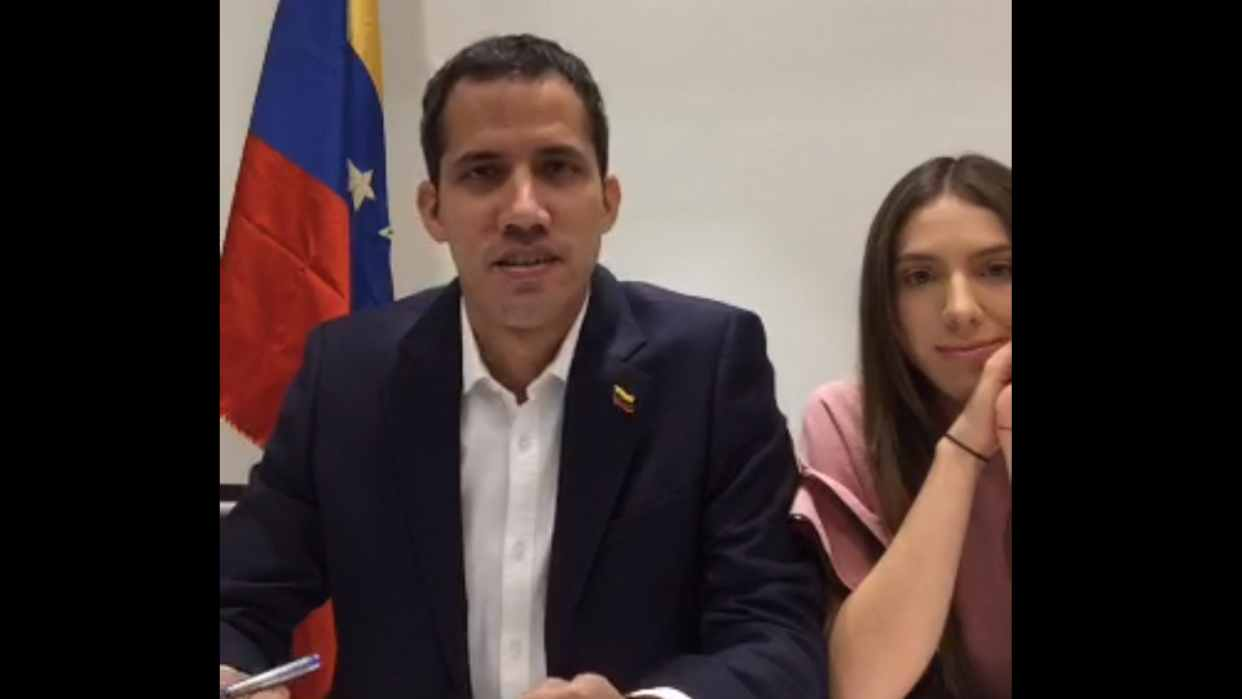
\includegraphics[width=300px]{EU_34709.jpg}%
\newline%
%
Caracas.{-}El presidente de la Asamblea Nacional (AN), Juan Guaidó, quien es reconocido como primer mandatario encargado de la República por más de medio centenar de países, dejó la noche de este domingo los pasos a seguir en caso de sufrir una detención por parte del Gobierno en su regreso al país que está previsto para este lunes.%
\newline%
%
"Si el régimen intenta secuestrarme (…) hemos dejado muy claro los pasos a seguir, en el corto plazo movilización (...) También tiene que ver con claras instrucciones a nuestros aliados internacionales, hermanos parlamentarios de todo el mundo. Hoy estamos mucho más unidos que nunca, mucho más movilizados que nunca, mientras nos mantengamos así ganamos, mientras que nos mantengamos así vamos hacia adelante", expresó Guaidó durante una trasmisión en vivo a través de las redes sociales.%
\newline%
%
"Estamos mucho más fuertes que nunca y no es momento de desfallecer", agregó el joven parlamentario, quien cruzó la frontera hacia Colombia el pasado 22 de febrero a pesar de contar con una medida de prohibición de salida del país dictada por el Tribunal Supremo de Justicia (TSJ) al que Guaidó considera ilegítimo por su designación y su falta de autonomía, pues son acusados por el Legislativo que preside de seguir las órdenes del Ejecutivo liderado por Nicolás Maduro.%
\newline%
%
Asimismo, reiteró a sus partidarios lo importante de la movilización enfatizando que este lunes todos deberían tomar las calles de Venezuela a partir de las 11 de la mañana. "En medio de la incertidumbre cuando más poderosa se vuelve la fe, fe en nosotros, un país que quería creer. Empezamos a creer en nosotros mismos, en unirnos, en movilizarnos y hoy estamos aquí más fuertes que nunca  ", expresó.%
\newline%
%
En Caracas llamó a una concentración en la Avenida Principal de Las Mercedes, al tiempo que indicó que en el interior del país los puntos serían anunciados por sus respectivos líderes.%
\newline%
%
Agradeció apoyo de los países de la región%
\newline%
%
Previamente, Guaidó agradeció el apoyo recibido en los países que visitó en su gira de esta semana que comprendió~Colombia, Brasil, Paraguay, Argentina y Ecuador.%
\newline%
%
A su vez, aseguró que esta lucha que adelanta junto a sus "compañeros" de la Asamblea Nacional "trasciende izquierdas y derechas".%
\newline%
%
Hizo referencia a los venezolanos radicados en dichas naciones. "Nuestra gira nos permitió escucharlos y sentir en carne propia sus ganas de regresar a casa", precisó al tiempo que reconoció "su esfuerzo incansable" no solo por intentar lograr sus metas en otros países ante la falta de oportunidades en el propio, sino que se han abrogado la manutención de sus familiares en Venezuela.%
\newline%
%
También planteó la posibilidad de que los empresarios venezolanos que han emigrado a otras latitudes vuelvan, creando un marco jurídico que fomente la inversión, lo que a su vez, en su opinión, se traduciría en fuentes de empleo para esos connacionales que decidan regresar al país.%
\newline%
%
Reiteró llamado a la FANB%
\newline%
%
Por otra parte, el joven parlamentario destacó el crecimiento "en la construcción de capacidades" al contar con el apoyo "de los venezolanos y el de la comunidad internacional"; sin embargo considera clave el apoyo de las Fuerzas Armadas para lograr "la restitución de la democracia" en el país.%
\newline%
%
En este sentido, advirtió que "la línea de mando está rota", pero a pesar de las manifestaciones que ha tenido a su favor y el número de militares que han demostrado su descontento al cruzar la frontera hacia Colombia o Brasil señaló que "debemos ser más, ser todos".%
\newline%
%
“Hoy la fuerza armada nacional bolivariana debe asumir su responsabilidad histórica, como lo hicieron esos oficiales que están en Cúcuta o los que están en Santa Elena de Uairén. Les pedimos que estén en Venezuela, que se pronuncien en bloque”, puntualizó.%
\newline%
%
Por eso reiteró su llamado a las FANB pidiéndoles que "no permitan que asesinos y hampones masacren a nuestros jóvenes e indígenas" y no crean en la supuesta intervención que denuncia Maduro que se fragua contra Venezuela pues, a su juicio, "la única intervención que existe en Venezuela es la cubana".%
\newline%
%
Por último, expresó que no puede existir paz "en un país donde masacran a nuestros indígenas, donde existen colectivos armados disparando a un pueblo desarmado que solo exige libertad", por lo que insistió en que deben colocarse del lado del pueblo y de la Constitución.%
\newline%
%
“El único que habla de guerra es Maduro. El dilema entre guerra y paz (…) evidentemente es un falso dilema todos queremos la paz (...) Nuestro dilema hoy en Venezuela es entre dictadura y democracia, entre pobreza y prosperidad y progreso, que solamente es posible cuando cese la usurpación”, argumentó.%
\newline%
%
\end{document}